\documentclass[11pt]{article}

%% MinionPro fonts 
%\usepackage[lf]{MinionPro}
%\usepackage{MnSymbol}
\usepackage{microtype}

%% Margins
\usepackage{geometry}
\geometry{verbose,letterpaper,tmargin=1in,bmargin=1in,lmargin=1in,rmargin=1in}

%% Other packages
\usepackage{amsmath}
\usepackage{amsthm}
\usepackage{amsfonts}
\usepackage[shortlabels]{enumitem}
\usepackage{titlesec}
\usepackage{soul}
\usepackage{tikz}
\usepackage{mathtools}
\usepackage{pgfplots}
\usepackage{tikz-3dplot}
\usepackage{algorithmic}
\usepackage[export]{adjustbox}
\usepackage{tcolorbox}
\usepackage{mathrsfs}
\usepackage{multicol}
\usepackage{framed}

%% Paragraph style settings
\setlength{\parskip}{\medskipamount}
\setlength{\parindent}{0pt}

%% Change itemize bullets
\renewcommand{\labelitemi}{$\bullet$}
\renewcommand{\labelitemii}{$\circ$}
\renewcommand{\labelitemiii}{$\diamond$}
\renewcommand{\labelitemiv}{$\cdot$}

%% Colors
\definecolor{rred}{RGB}{204,0,0}
\definecolor{ggreen}{RGB}{0,145,0}
\definecolor{yyellow}{RGB}{255,185,0}
\definecolor{bblue}{rgb}{0.2,0.2,0.7}
\definecolor{ggray}{RGB}{190,190,190}
\definecolor{ppurple}{RGB}{160,32,240}
\definecolor{oorange}{RGB}{255,165,0}

%% Shrink section fonts
\titleformat*{\section}{\normalsize\bf}
\titleformat*{\subsection}{\normalsize\bf}
\titleformat*{\subsubsection}{\normalsize\it}

% %% Compress the spacing around section titles
\titlespacing*{\section}{0pt}{1.5ex}{0.75ex}
\titlespacing*{\subsection}{0pt}{1ex}{0.5ex}
\titlespacing*{\subsubsection}{0pt}{1ex}{0.5ex}

%% amsthm settings
\theoremstyle{definition}
\newtheorem{problem}{Problem}
\newtheorem{example}{Example}
\newtheorem*{theorem}{Theorem}
\newtheorem*{bigthm}{Big Theorem}
\newtheorem*{biggerthm}{Bigger Theorem}
\newtheorem*{bigcor1}{Big Corollary 1}
\newtheorem*{bigcor2}{Big Corollary 2}

%% tikz settings
\usetikzlibrary{calc}
\usetikzlibrary{patterns}
\usetikzlibrary{decorations}
\usepgfplotslibrary{polar}

%% algorithmic setup
\algsetup{linenodelimiter=}
\renewcommand{\algorithmiccomment}[1]{\quad// #1}
\renewcommand{\algorithmicrequire}{\emph{Input:}}
\renewcommand{\algorithmicensure}{\emph{Output:}}

%% Answer box macros
%% \answerbox{alignment}{width}{height}
\newcommand{\answerbox}[3]{%
  \fbox{%
    \begin{minipage}[#1]{#2}
      \hfill\vspace{#3}
    \end{minipage}
  }
}

%% \answerboxfull{alignment}{height}
\newcommand{\answerboxfull}[2]{%
  \answerbox{#1}{6.38in}{#2} 
}

%% \answerboxone{alignment}{height} -- for first-level bullet
\newcommand{\answerboxone}[2]{%
  \answerbox{#1}{6.0in}{#2} 
}

%% \answerboxtwo{alignment}{height} -- for second-level bullet
\newcommand{\answerboxtwo}[2]{%
  \answerbox{#1}{5.8in}{#2}
}

%% special boxes
\newcommand{\wordbox}{\answerbox{c}{1.2in}{.7cm}}
\newcommand{\catbox}{\answerbox{c}{.5in}{.7cm}}
\newcommand{\letterbox}{\answerbox{c}{.7cm}{.7cm}}

%% Miscellaneous macros
\newcommand{\tstack}[1]{\begin{multlined}[t] #1 \end{multlined}}
\newcommand{\cstack}[1]{\begin{multlined}[c] #1 \end{multlined}}
\newcommand{\ccite}[1]{\only<presentation>{{\scriptsize\color{gray} #1}}\only<article>{{\small [#1]}}}
\newcommand{\grad}{\nabla}
\newcommand{\ra}{\ensuremath{\rightarrow}~}
\newcommand{\maximize}{\text{maximize}}
\newcommand{\minimize}{\text{minimize}}
\newcommand{\subjectto}{\text{subject to}}
\newcommand{\trans}{\mathsf{T}}
\newcommand{\bb}{\mathbf{b}}
\newcommand{\bx}{\mathbf{x}}
\newcommand{\bc}{\mathbf{c}}
\newcommand{\bd}{\mathbf{d}}

%% LP format
%    \begin{align*}
%      \maximize \quad & \mathbf{c}^{\trans} \mathbf{x}\\
%      \subjectto \quad & A \mathbf{x} = \mathbf{b}\\
%                       & \mathbf{x} \ge \mathbf{0}
%    \end{align*}

%Space between rows:
%\def\arraystretch{2.2}
%
%Space between columns:
%\arraycolsep=1.4pt


%% Redefine maketitle
\makeatletter
\renewcommand{\maketitle}{
  \noindent SA405 -- AMP \hfill Rader \S 14.1, 14.2  \\

  \begin{center}\Large{\textbf{\@title}}\end{center}
}
\makeatother

%% ----- Begin document ----- %%
\begin{document}
  
\title{Lesson 17.  Branch-and-bound}

\maketitle

%%%
\section{Today...}
\begin{itemize}
\item ``Combinatorial Explosion'' of IPs
\item Branch-and-bound for solving IPs
\end{itemize}

%\renewcommand\labelitemi{--}
\section{``Combinatorial Explosion'' of IPs}

Consider the knapsack problem (with all nonegative parameters) in which we choose the most valuable collection of items to fit into a limited size ``knapsack'':

    \begin{align*}
      \maximize \quad & \sum_{i=1}^n c_i x_i \\
      \subjectto \quad & \sum_{i=1}^n a_i x_i \leq b \\
                       & x_i \in \{0,1\}, \text{ for } i = 1, 2,\dots,n,
    \end{align*}
\begin{itemize}
\item decision variable $x_i = \letterbox~$ if we choose to pack item $i$, $x_i = \letterbox$ otherwise;
\item $c_i$ represents the \wordbox of item $i$;
\item $a_i$ represents the \wordbox of item $i$;
\item $b$ represents the \wordbox of the knapsack.
\end{itemize}

\bigskip
\begin{problem}
Suppose $n = 5$.  
\begin{enumerate}[(a)]
\item Write one possible solution to the knapsack problem. $(x_1, x_2, x_3, x_4, x_5) =$ \wordbox
\item Which items does your solution recommend that you pack?  

\answerboxone{c}{1cm}

\item If the constraint eliminates half of the possible solutions, how many feasible solutions are there?  

\answerboxone{c}{1cm}
\end{enumerate}
\end{problem}

%%%
\newpage

\begin{tcolorbox}
\textbf{Complete enumeration} is a solution strategy for the knapsack problem (or any bounded IP) in which 
\begin{itemize}
\item the objective value is computed for \emph{every feasible solution};
\item the solution with the maximum objective function value is chosen as the optimal solution.
\end{itemize}
\end{tcolorbox}

Now suppose $n = 100$ (a moderately-sized problem) and that the knapsack constraint eliminates half of the possible solutions.  In a \textbf{complete enumeration} strategy in which we can check \emph{one billion solutions per second},

\begin{itemize}
\item there are 
\begin{center}
\catbox $\approx 6.3 \times 10^{29}$
\end{center}
feasible solutions to check,
\item requiring about 

\begin{center}
$6.3 \times 10^{20}$ seconds $~\approx~~$ \wordbox ~years
\end{center}
for complete enumeration.
\end{itemize}

\begin{tcolorbox}
In general, for even moderately-sized problems, \textbf{complete enumeration} is a totally (AWESOME or HOPELESS) solution strategy.
\end{tcolorbox}

And this is why we have branch-and-bound...

%%%%%
\vfill
\section{Branch-and-bound for solving IPs}

\begin{tcolorbox}
\textbf{Branch-and-bound} is an algorithm for solving mixed-integer programs: 
\begin{itemize}
\item the feasible region is iteratively subdivided to create smaller subproblems  (``branching'' phase);
\item the subproblems are bounded by solving relaxations  (``bound'' phase).
\end{itemize}
\end{tcolorbox}

Typically, modern IP (or MIP) solvers use some variation of branch-and-bound.
\vfill
%%%
\newpage
\subsection{Branching a subproblem on a variable}

To \textbf{branch} means to split a problem into two smaller subproblems. 

\begin{itemize}
\item For example, to find the tallest midshipman in the brigade:
\begin{itemize}
\item solve subproblem 1:  \answerbox{c}{10cm}{.7cm}
\item solve subproblem 2:  \answerbox{c}{10cm}{.7cm}
\item compare these two solutions.
\end{itemize}

\item  The union of the feasible regions (FRs) of the subproblems should be \wordbox the FR of the original problem.
\item For example, consider the IP below:
    \begin{align*}
    (P1) ~~~ z_{IP}^* = & \text{ max } 8x + 7y\\
      \text{s.t.} \quad & -18x + 38y \leq 133\\
                       & 13x + 11y \leq 125\\
                       & 10x -    8y \leq 55\\
                       & x, y \in \mathbb{Z}^{\geq 0}
    \end{align*}
Find an upper bound for $z_{IP}^*$ by solving the LP relaxation of (P1).  Suppose the LP relaxation has optimal solution $(x, ~y) =  (4.75, ~5.75)$ with optimal objective value $z^*_{LP} = 78.25$.  This provides the following bound on $z_{IP}^*$:
\[ z^*_{IP} ~\leq~ \catbox \]
%\[ z^*_{IP} ~\leq~ \lfloor z^*_{LP} \rfloor ~=~ \lfloor 78.25 \rfloor ~=~ 78, ~~~\text{ where }~
%(x,~y) = (4.75, ~5.75). \]

\bigskip
\begin{itemize}
	\item Since the optimal LP solution, \underline{\hspace{3cm}}, is not integer-valued, we must \textbf{branch on one of the fractional-valued variables}.  Let's choose to \textbf{branch on $x$}.
 	\item  We know that $x$ must be integer-valued, so we can eliminate all the fractional values between 4 and 5.  Our two subproblems leverage this fact:
\end{itemize}

\begin{minipage}{0.5\textwidth}
\hspace{1.3cm}$x$ must no more than 4 or...
    \begin{align*}
    (P2) ~~~ z_{IP}^* = & \text{ max } 8x + 7y\\
      \text{s.t.} \quad & -18x + 38y \leq 133\\
                       & 13x + 11y \leq 125\\
                       & 10x -    8y \leq 55\\
                       & \wordbox \\
                       & x, y \in \mathbb{Z}^{\geq 0}
    \end{align*}
\end{minipage}
\begin{minipage}{0.5\textwidth}
\hspace{1.3cm}at least 5.
    \begin{align*}
    (P3) ~~~ z_{IP}^* = & \text{ max } 8x + 7y\\
      \text{s.t.} \quad & -18x + 38y \leq 133\\
                       & 13x + 11y \leq 125\\
                       & 10x -    8y \leq 55\\
                       & \wordbox \\
                       & x, y \in \mathbb{Z}^{\geq 0}
    \end{align*}
\end{minipage}


%%%
\newpage
\item Continuing the previous example, the \emph{relaxed} feasible region of (P1) is shown below.
Sketch the \emph{relaxed} feasible regions of (P2) and (P3):

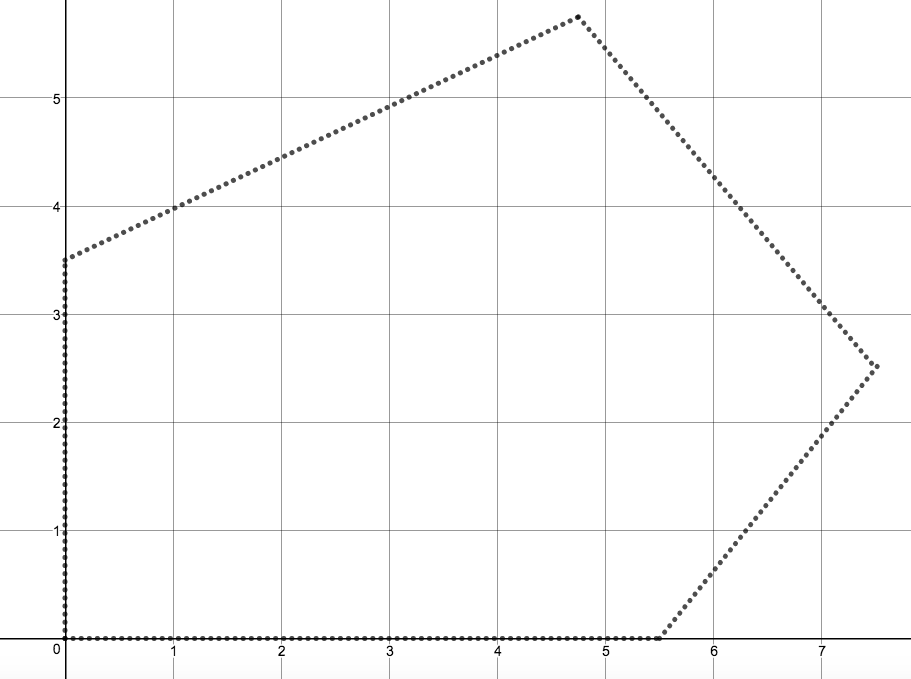
\includegraphics[width=0.4\textwidth]{fr} 


\item  In order to make progress in branch-and-bound: 

The union of the \emph{relaxed} FRs of the subproblems should be a \wordbox subset of the \emph{relaxed} FR of the original problem.  (I.e., we \emph{tighten} our formulation as we go.)

\end{itemize}

\subsection{Branch-and-bound terminology}
\begin{itemize}
\item As we branch on integer variables, we keep track of progress in a \textbf{branch-and-bound} \catbox.  \textbf{Nodes} represent \wordbox to the LP \wordbox.
%	\begin{itemize}
%		\item    
%		\begin{itemize} 
%			\item \textbf{root node} is the original problem. 
%			\item subproblem nodes are the ``children'' of a ``parent'' node.
%		\end{itemize}
%		\item \textbf{directed edges} represents the way parent problems change to become subproblems
%	\end{itemize}
\item At some point during the algorithm, we will encounter an \emph{integer feasible} solution which becomes the \textbf{incumbent solution}. 
	\begin{itemize}
		\item The incumbent solution provides a (LOWER~/~UPPER) bound on the global maximum.
		\item If later we find a (BETTER~/~WORSE) feasible solution, it becomes the new incumbent solution.
		\begin{tcolorbox} The \textbf{incumbent solution} is the \catbox feasible solution found so far. \end{tcolorbox}
	\end{itemize}
\item To \textbf{fathom} (or \textbf{prune}) a node means to eliminate its subproblem from consideration.  
\begin{itemize}
	\item We know this part of the feasible region (CONTAINS ~/~ DOES NOT CONTAIN) the optimal solution.)  
\end{itemize}
%\begin{tcolorbox}
%We can \textbf{prune} a node representing subproblem (SP) in the following situations:
%	\begin{enumerate}[(1)]
%		\item  (SP) is \wordbox.
%		\item  The upper bound on (SP) is \wordbox than the global lower bound provided by the current incumbent solution.  (I.e., the incumbent solution is better than any solution in (SP).)
%The overall strategy of branch-and-bound is to iteratively branch on integer variables, at each stage increasing the number of integer variables in the relaxed solution.
%	\end{enumerate}
%\end{tcolorbox}
%\item A node is \textbf{active} if it has neither been fathomed nor branched.
\item Leaf nodes are (BRANCHED ~/~ UNBRANCHED) nodes.  

There are 3 types of \textbf{leaf nodes}.
	\begin{enumerate}[(1)]
		\item \wordbox %\textbf{fathomed}
		\item contains \textbf{current \wordbox solution} (only one of these nodes!)
		\item \textbf{active} -- still requires branching
	\end{enumerate}

\end{itemize}

\newpage
\subsection{Algorithm}

\begin{tcolorbox}
\textbf{Branch-and-bound for solving IPs}

\bigskip
\textbf{(Initialize)}
\begin{itemize}
\item The root node (original problem) is the only active node.  
\item Set global lower bound: $\underline{z} = -\infty$.  There is no incumbent solution $\underline{x}$ to start.
\end{itemize}

\bigskip
\textbf{(Iterate)}
\begin{itemize}
\item Select an \textbf{active} node.  Branch on a \textbf{fractional} variable to create two subproblems.

\item For each subproblem (SP):

- Solve its relaxation (LP), if possible, for optimal solution $x$ with objective value $z$:
\renewcommand\labelitemii{}
\begin{itemize} 
	\item (LP) infeasible $\Rightarrow$ \textbf{fathom} (SP).
	\item $z \leq \underline{z}$ $\Rightarrow$ \textbf{fathom} (SP).
	\item $z > \underline{z}$:
\renewcommand\labelitemiii{}
	\begin{itemize}
		\item $x$ integer $\Rightarrow$ $x$ becomes new \textbf{incumbent solution}: $\underline{x} = x$, $\underline{z} = z$.

 ~~~~~~~~~~~~~~~~~\textbf{Fathom} nodes whose upper bounds are less than the new $\underline{z}$.
		\item $x$ fractional $\Rightarrow$ (SP) becomes \textbf{active} with local upperbound $\lfloor z \rfloor$.
	\end{itemize}

\end{itemize}
\end{itemize}

\bigskip
\textbf{(Stopping condition)}
\begin{itemize}
\item When there are no more active nodes, the incumbent solution is the optimal solution to the original problem.
\end{itemize}
\end{tcolorbox}

\bigskip
\textbf{MIP gap}

Another common stopping criterion is a predetermined ``MIP gap'', which is a measure of how close the current global lower bound, LB, and global upper bound, UB, are, as a fraction of the LB:
\[
MIP~gap =   \answerbox{c}{3cm}{2cm} %\frac{|UB-LB|}{|LB|}.
\]

When the MIP gap is small, the current incumbent solution is guaranteed to be \emph{close} to optimal.  For hard problems, we can tell the solver to stop at a ``good'' solution by setting a MIP gap flag.  In Pyomo, this looks like:
\begin{center}
\texttt{pyo.SolverFactory(`glpk').solve(model, \wordbox)} %mipgap=0.01
\end{center}

\newpage
\textbf{Branch-and-bound Example}  

To demonstrate the branch-and-bound algorithm, we will work through an example using the following  documents:

\begin{itemize}
\item  L17\_Branch\_And\_Bound\_Example.pdf
\item  L17\_Branch\_And\_Bound\_Example.ipynb
\end{itemize}

%%%

\bigskip

\textbf{Branching Rules}

The procedure in the box on the previous page is really an \emph{algorithmic framework}, rather than an actual algorithm. To become a true algorithm, we would need to specify
\begin{itemize}
\item a \textbf{branching rule} (to decide which \wordbox node to branch);
\item a \textbf{variable selection rule} (to decide which \wordbox variable to branch on).
\end{itemize}

\begin{tcolorbox}
\textbf{Possible branching rules}: 
\begin{itemize}
\item \textbf{depth-first search:} Quickly go deep in the tree by always branching on one of the most recently constructed active nodes, for example.
	\begin{itemize}
		\item ADVANTAGE:  We get an \wordbox solution quickly, which we require in order to fathom feasible nodes.
		\item DISADVANTAGE:  Long computation times, if we keep diving down to feasible solutions in every successive subproblem.
	\end{itemize}
\item \textbf{best-first search:} Branch on the active node with the \wordbox \emph{local upper bound}.
	\begin{itemize}
		\item ADVANTAGE:  We explore promising regions early on.
		\item DISADVANTAGE:  It may take a long time to get a first incumbent solution.  It also tends to produce a very wide tree, requiring a lot of memory to maintain many active nodes.
	\end{itemize}
\item a \textbf{hybrid approach} is most common.  For example, use depth-first to get an incumbent solution.  Switch to best-first to search promising nodes.  
\end{itemize}
\end{tcolorbox}

\newpage
\subsection{Branch-and-bound variations}
In reality, modern MILP solvers build on the basic b-and-b framework presented here.

Most solvers attain a \textbf{lower-bounding feasible solution in every subproblem} by solving a \emph{restriction} of the subproblem (rather than a relaxation).  The best of these feasible solutions is maintained as the incumbent solution.

Most IP/†MIP solvers employ a variation of branch-and-bound called \textbf{branch-and-cut}.  In some subproblems, new constraints are generated in a ``cutting-plane'' phase to tighten the formulation of the subproblem relaxation (LP).  This results in 
	\begin{itemize}
		\item a \emph{less fractional} optimal solution $x$ to the subproblem (LP);
		\item a \emph{tighter upperbound} $z$ on the subproblem;
		\item \emph{fewer branching nodes} overall.
	\end{itemize}


\end{document}


